\chapter{Fundamentação Teórica}
Nesse capítulo, primeiro apresentaremos uma visão geral das redes neurais artificiais, desde o neurônio artificial, os principais tipos de arquitetura e chegando até os autocodificadores variacionais.
No segundo momento, fundamentamos brevemente a teoria de compressão de dados, medida de informação e representação de imagens. Por fim, explicamos o funcionamento do \acrshort{jpeg}  e citamos as principais métricas objetivas para avaliar a qualidade entre imagens.    

\section{Redes Neurais Artificiais}
Nessa seção, descrevemos a ideia básica de qualquer \gls{rna}, suas vantagens e seu elemento essencial: o neurônio artificial. 

%paradigma de programação capaz de encontrar representações úteis dos dados de entrada para facilitar tarefas de classificação e regressão. 

O aprendizado de máquina, do inglês \textit{machine learning}, é um campo de conhecimento interdisciplinar que refere-se à detecção automatizada de padrões significativos nos dados através da construção de programas de computador que melhoram com a experiência (aprendizagem) \cite{shalev2014understanding}. 
Na etapa de aprendizado, o modelo de aprendizagem de máquina  utiliza os dados de entrada para realizar predições dos resultados. Uma medida de erro é calculado entre a previsão e o resultado esperado. Essa medição é usada como um sinal de retroalimentação (\textit{feedback}) para ajustar as regras  do algoritmo de modo a minimizar o erro. Após o aprendizado do modelo ele deve ser capaz de fazer inferências com novos exemplos dos dados de entrada \cite{FrancoisDeepLearning}.

Na programação clássica, os seres humanos inserem regras (um programa) e dados a serem processados de acordo com essas regras para obter as respostas  -  não há processo de aprendizado. A figura em \ref{fig:machinelearning} resume a diferença essencial entre a programação convencional e o aprendizado de máquina \cite{FrancoisDeepLearning}.  


\begin{figure}[h]
	\centering
	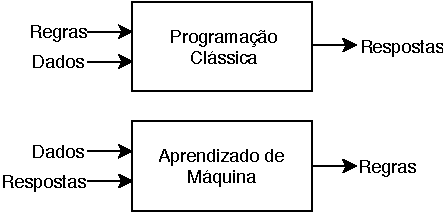
\includegraphics[width=0.4\textwidth]{figuras/MachineLearning.pdf}
	\caption[Paradigmas de programação]{Aprendizado de Máquina: um novo paradigma de programação. Adaptado de \cite{FrancoisDeepLearning}.}
	\label{fig:machinelearning}
\end{figure}


As \acrshort{rna}'s são técnicas específicas de aprendizado de máquina inspiradas no funcionamento do cérebro humano. A semelhança com esse órgão humano advém de dois aspectos principais \cite{Haykin}:
\begin{enumerate}
	\item O conhecimento é adquirido pela rede a partir do seu ambiente através de um processo de aprendizagem;
	\item Forças de conexão de neurônios, conhecidos como pesos sinápticos, são utilizados para armazenar o conhecimento adquirido.
\end{enumerate}

Na literatura, o termo aprendizado profundo (\textit{deep learning}) é usado para se referir às redes neurais com muitas camadas de processamento \cite{lecun2015deep,bengio2009learning}. Uma camada consiste em um módulo que realiza uma transformação matemática sobre uma entrada e gera um conjunto de dados de saída. Os pesos são os valores numéricos responsáveis por parametrizar as transformações em cada camada \cite{FrancoisDeepLearning}. 
As camadas são conectadas em cadeia (uma após a outra) de forma que a última camada forneça uma representação numérica útil para o modelo realizar as predições. Após a previsão, a função de perdas calcula  um valor do quão bem as previsões da rede correspondem ao esperado. Tal valor é usado por um algoritmo de otimização (otimizador) para realizar a atualização dos pesos. 
O aprendizado ou treinamento de uma \acrshort{rna} usando amostras dos dados e os seus respectivos rótulos é denominado de aprendizado supervisionado. A  Figura \ref{fig:modeloRNA} apresenta um esquemático do procedimento para o treinamento de uma rede neural artificial de 2 camadas.

\begin{figure}[h]
	\centering
	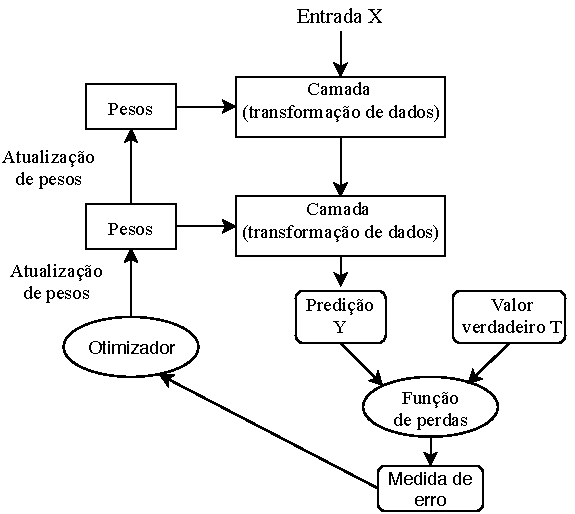
\includegraphics[width=0.6\textwidth]{figuras/modeloRNA.pdf}
	\caption[Principais componentes em uma \acrshort{rna}]{A rede neural composta por 2 camadas encadeadas mapeia os dados de entrada para as previsões. A função de perdas compara essas previsões às metas, produzindo um valor de erro. O otimizador usa esse valor para atualizar os pesos da rede. Adaptado de \cite{FrancoisDeepLearning}.}
	\label{fig:modeloRNA}
\end{figure}


O neurônio artificial, também chamado perceptron, é a unidade básica de processamento de uma rede neural e a interligação em massa dessas unidades computacionais a permite alcançar desempenho cada vez melhor \cite{Haykin}.  As principais propriedades úteis das \acrshort{rna}'s em diversas tarefas de tomada de decisão são \cite{Haykin}:
\begin{enumerate}
	\item A possibilidade de não linearidade dos neurônio, o que permite a rede resolver problemas não-lineares e complexos;
	\item  Adaptabilidade: os pesos das \acrshort{rna}'s são facilmente adaptados sendo possível retreinar uma rede em um novo ambiente com pequenas modificações em relação ao original. Ademais, é possível encontrar um equilíbrio para que os pesos sejam modificados se a fonte de dados é não-estacionária e capaz de ignorar perturbações espúrias;
	\item Resposta a evidência: nas tarefas de classificação a rede pode ser projetada para indicar o grau de certeza nas suas previsões. Isso permite ao modelo descartar informações ambíguas e aprimorar a performance de classificação;
	\item Informação contextual: cada neurônio é potencialmente afetado pelo comportamento dos demais de forma a proporcionar um conhecimento de contexto ao modelo.
\end{enumerate}



\subsection{Neurônio Artificial}
O neurônio é a unidade mais básica da \acrshort{rna}. O seu modelo está ilustrado na Figura \ref{fig:neuronio}.

\begin{figure}[h]
	\centering
	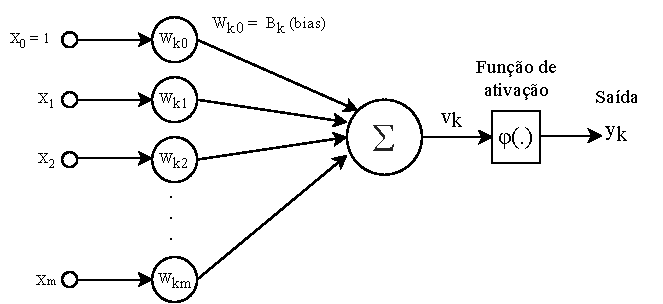
\includegraphics[width=0.6\textwidth]{figuras/neuronio.pdf}
	\caption[Modelo do neurônio matemático.]{Representação do neurônio artificial formado por um vetor de peso $W$ de tamanho $m$. A entrada $X_0$ é artificial e o peso associada a ela é denominado viés. O neurônio funciona como um operador matemático simples que realiza um mapeamento de muitos para 1. Adaptado de \cite{Haykin}.}
	\label{fig:neuronio}
\end{figure}

A sua descrição matemática é dada pelas seguintes equações.

\begin{equation}
\begin{aligned}
\centering    
v_{k} = \sum_{j=0}^{m}w_{kj}x_{j} 
\end{aligned}
\end{equation}


\begin{equation}
\begin{aligned}
\centering    
y_{k} = \phi(v_{k})
\end{aligned}
\end{equation}

Em que $x_{0}$ é uma entrada fictícia que será multiplicada pelo viés ou do inglês \textit{bias}, $w_{k0} = b_{k}$; $x_{1},x_{2}, ...,x_{m}$ são os valores reais de entrada, $w_{k1},x_{k2}, ...,x_{km}$ são os pesos sinápticos do neurônio k; $v_{k}$ é a saída do produto escalar entre os vetores $\textbf{w}$ e $ \textbf{x}$;  $\phi()$ é denominada função de ativação e $y_{k}$ é o sinal de saída do neurônio. O viés é um termo independente dos sinais de entrada e tem o objetivo de fornecer mais um grau de liberdade ao neurônio.

\subsubsection{Funções de ativação}
A função de ativação é uma transformação matemática adicional que ocorre no perceptron. O seu uso permite a solução de problemas complexos e não-lineares, tais como tarefas de visão computacional e processamento de linguagem natural \cite{Mitchell}. 
O neurônio com a função limiar foi utilizado no primeiro modelo de perceptron \cite{mcculloch1943logical,Haykin} e contém a propriedade ``tudo ou nada''.  As funções com formato de S e não-lineares são chamadas de sigmóides e amplamente usadas em \acrshort{rna}'s. Entre elas há a função logística que restringe a saída no intervalo [0,1] e a tangente hiperbólica cuja saída pertence ao intervalo [-1,1]. Elas são usadas em neurônios das camadas intermediárias ou na última para problemas de classificação binária ou regressão. 
A função \textit{softmax} também é uma função sigmóide usada para prever as probabilidades associadas a uma classificação multi-classe \cite{Goodfellow2016}.  Ela toma um vetor $K$-dimensional correspondentes aos $K$ neurônios de uma camada e produz outro vetor $K$-dimensional com valores reais no intervalo (0, 1) que somam 1.  A função \textit{softmax} é idealmente usada na camada de saída do classificador \cite{Goodfellow2016}.
A \gls{relu} \cite{nair2010rectified}, é uma função não-linear que mapeia uma entrada para zero se ela for negativa ou retorna a própria entrada se ela for positiva. Diferentemente das funções sigmóides, ela é uma função não saturada e em decorrência disso possui duas vantagens principais: minimiza o problema denominado “gradiente de explosão e fuga” e acelerar a velocidade de convergência da rede \cite{xu2015empirical}.
As equações das funções de ativações mencionadas aqui e a suas derivadas estão apresentadas na Tabela \ref{table:func_ativacoes}. 

\begin{table}[htbp]
	\centering
	
	\caption{Funções de ativações usadas em redes neurais artificiais e suas respectivas derivadas. Todas são funções de uma variável, exceto a função \textit{softmax} que atua em um conjunto de entrada e retorna um grupo de saída.}
	{\renewcommand{\arraystretch}{2.5}
		\begin{tabular}{|l|l|l|}
			\hline
			\textbf{Função de ativação} & \textbf{Equação} & \textbf{Derivada} \\ \hline
			Limiar & \(\displaystyle \beta(v) =  \begin{cases} 1 ,  &\text{se $v \geq  0$}; \\ \text{0},  & \text{se $v <0$} \end{cases}\) & \(\displaystyle \beta'(v) =  \begin{cases} 0 ,   & \text{se $v \neq 0$} \\ \text{Não definida},  &   \text{se $v = 0$} \end{cases}\) \\ \hline
			Logística & \(\displaystyle   \alpha (v) =  \frac{\mathrm{1} } {\mathrm{1} + e^{-v}}\) & \(\displaystyle\alpha'(v) =  \alpha(v) \times (1 - \alpha(v)\) \\ \hline
			Tangente Hiperbólica & \(\displaystyle tanh(v) =  \frac{e^{v} - e^{-v} }{ e^{v} + e^{-v}}\) & \(\displaystyle tanh'(v) = 1 -tanh^{2}(v) \) \\ \hline
			\text{\acrshort{relu}} & \(\displaystyle relu(v) =  \begin{cases} v , &\text{ se $v \geq 0$;} \\ \text{0},  &\text{se $ v <0$}  \end{cases}\) & \(\displaystyle relu'(v) =  \begin{cases} 1 , &\text{ se $v > 0$} \\ \text{0},  &\text{se $ v <0$}  \end{cases}\) \\ \hline
			\textit{Softmax} & \(\displaystyle  S(\textbf{v})_j = \frac{e^{v_j}}{\sum^{K}_{k=1}e^{v_k} }\)   & \(\displaystyle \frac{\partial S_j}{\partial v_i} =  \begin{cases} S_j(1-S_i), &\text{ se $i = j$} \\ -S_jS_i,  &\text{se $i \neq  j$}  \end{cases}\) \\ \hline
	\end{tabular}} \quad
	\label{table:func_ativacoes}
\end{table}

%\subsubsection{Aprendizado}

O processo de aprendizado de uma rede neural consiste em determinar um vetor de pesos que seja capaz de prever corretamente a saída $y$ para o máximo dos exemplos de treinamento fornecidos \cite{Mitchell}. Além disso, o modelo deve ser geral o suficiente para realizar previsões corretamente em novos exemplos. 
Esse processo pode ser alcançado através dos algoritmos de retropropagação (conhecido do  inglês como \textit{backpropagation}) \cite{rumelhart1988learning, Goodfellow2016} e de descida do gradiente. O primeiro toma a medida do erro, calculado na saída da rede neural, e computa o seu gradiente em relação a cada um dos pesos da rede \cite{Goodfellow2016}. O segundo é usado para atualizar os pesos por meio do gradiente calculado  \cite{Mitchell}.  A descida do gradiente é um algoritmo específico dos otimizadores.  
A seguir, apresentamos a atuação desses algoritmos no treinamento do neurônio artificial.  A Equação \ref{eq:erro_neuronio} é uma função de perdas relativa aos exemplos de treinamento \cite{Mitchell}.

\begin{equation}
\label{eq:erro_neuronio}
\begin{aligned}
\centering    
E(\textbf{w}) = \displaystyle \frac{1}{2}\sum_{d=0}^{D}( t_{d} - y_{d})^{2}  
\end{aligned}
\end{equation}

Onde, D é o conjunto de exemplos de treinamento, $t_{d}$ é a saída de destino para o exemplo de treinamento d e $y_{d}$ é a predição do perceptron. Por essa definição, caracterizamos $E$ como uma função de $\textbf{w}$ \cite{Mitchell}.
A Figura \ref{fig:gradiente} ilustra a superfície do erro hipotético em função do espaço de hipóteses para o vetor de pesos de tamanho igual a 2. O espaço de hipótese é formado pelo plano $w_0w_1$ enquanto o erro para cada vetor de pesos está no eixo vertical. Para qualquer ponto nessa superfície o algoritmo de descida de gradiente indica a direção de redução mais acentuada do erro. Com essa informação o vetor de pesos é atualizado sucessivamente até encontrar um mínimo na superfície de possibilidades do erro. Idealmente, desejamos que esse o mínimo seja o global, entretanto para muitas situações não há como garantir isso \cite{Mitchell}. 

\begin{figure}[h]
	\centering
	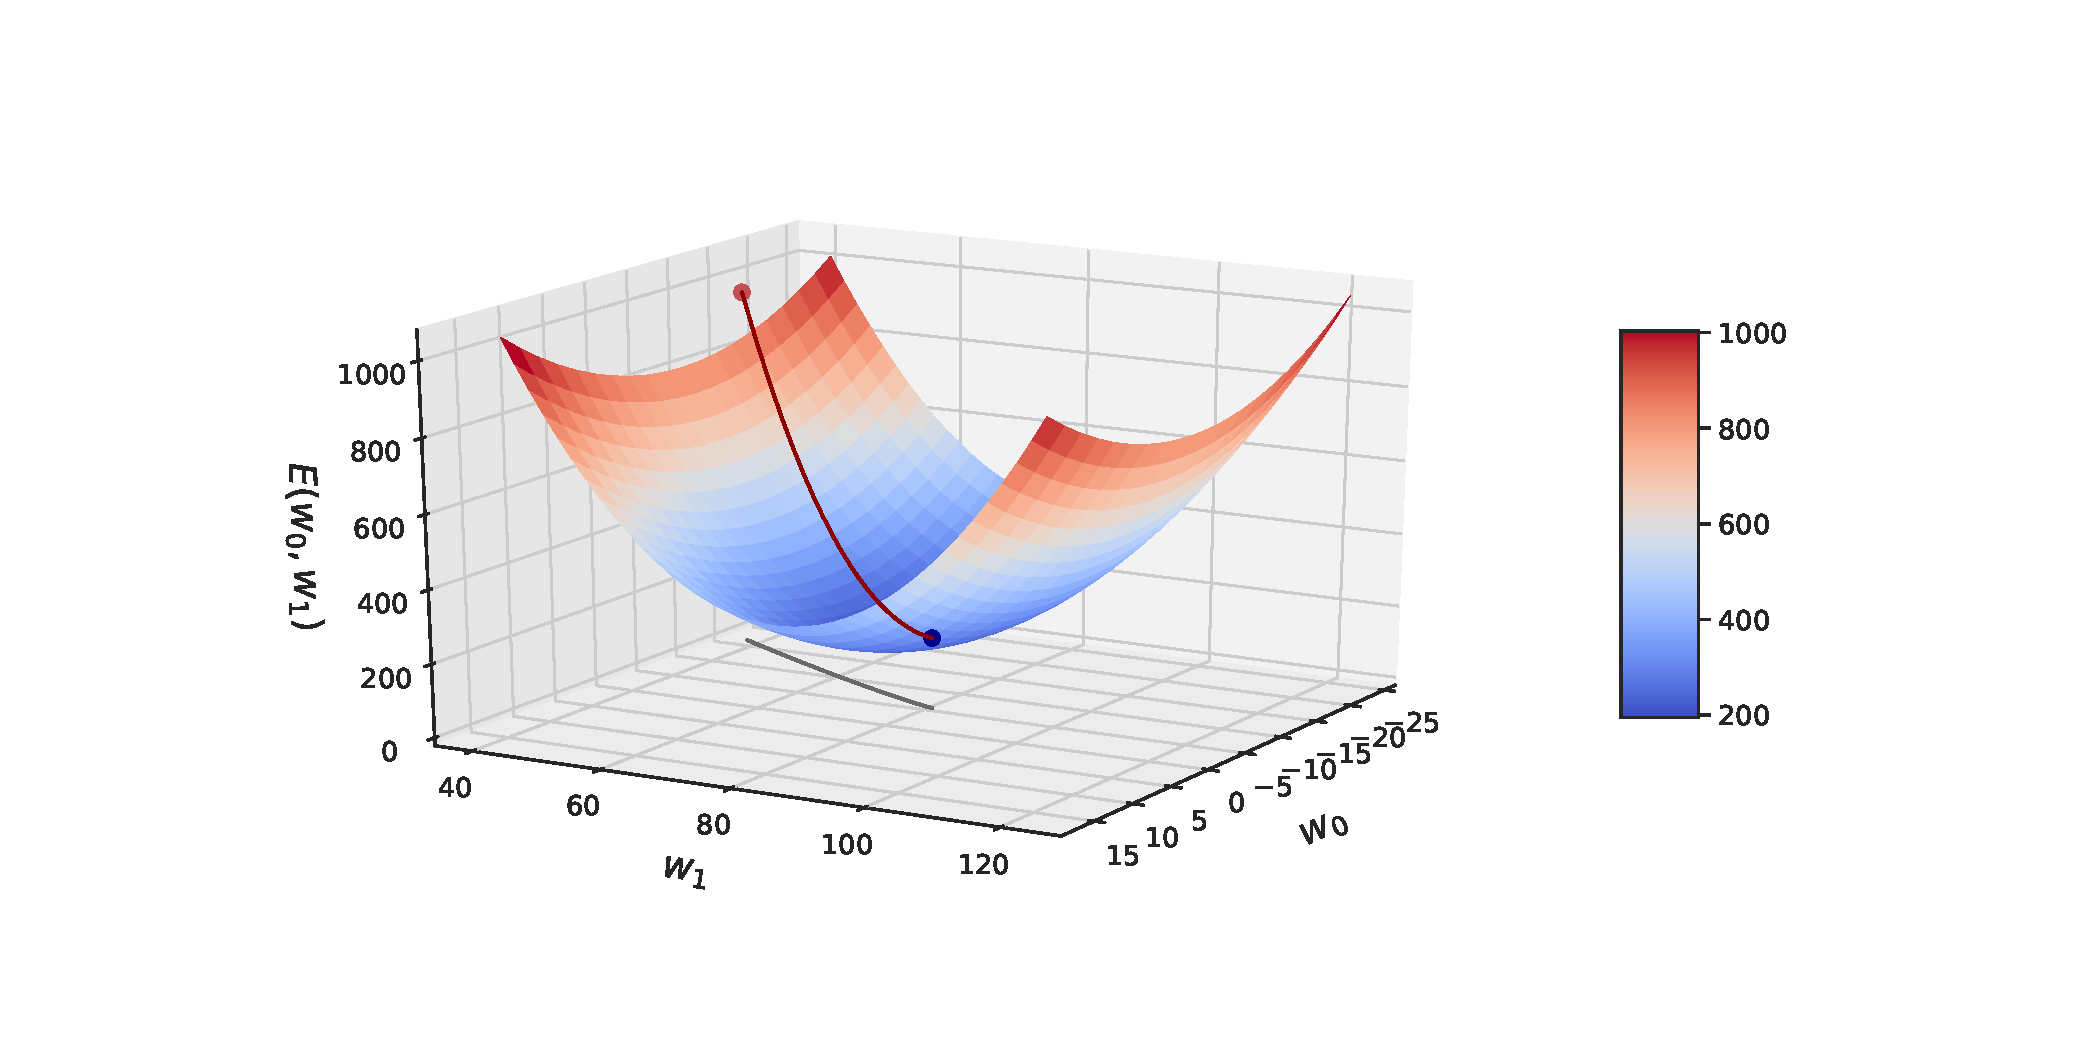
\includegraphics[width=1.1\textwidth]{figuras/gradient_descent.eps}
	\caption[Superfície de erro para o aprendizado dos pesos de um neurônio simples.]{Visualização do espaço de hipóteses dos pesos e atuação do algoritmo de descida de gradiente. Os pontos vermelho e azul indicam o início e o fim do aprendizado, respectivamente. A linha cinza é a projeção da curva de aprendizado no plano $w_0w_1$.}
	\label{fig:gradiente}
\end{figure}

A direção de maior crescimento de uma função é obtido pelo cálculo do vetor gradiente em relação às variáveis independentes. No neurônio artificial, o algoritmo de retropropagação obtém esse vetor de forma direta, conforme a próxima equação. 

\begin{equation}
\begin{aligned}
\nabla E(\textbf{w}) \equiv \left [ \frac{\partial E}{\partial w_{0}}, \frac{\partial E}{\partial w_{1}},...,\frac{\partial E}{\partial w_{m}} \right]
\end{aligned}
\end{equation}

Portanto, o negativo do vetor $\nabla E(\textbf{w})$ informa a direção de maior decaimento do erro e a regra de treinamento para a descida do gradiente é:

\begin{equation}
\begin{aligned}
\textbf{w}^{t+1}   &= \textbf{w}^{t} + \Delta(\textbf{w}^{t} ) \\
\Delta(\textbf{w}^{t}) &= - \eta \times \nabla E(\textbf{w}^{t})
\end{aligned}
\end{equation}

Nessa equação, o subíndice é usado para diferenciar o vetor de pesos atual, $\textbf({w}^{t})$, do próximo $\textbf({w}^{t+1})$. O parâmetro $\eta>0$ é a taxa de aprendizado, responsável por controlar o tamanho do passo da atualização dos pesos. O sinal negativo é empregado para obter o sentido oposto ao vetor gradiente. Essa regra de treinamento também pode ser escrita para cada componente do vetor de pesos:

\begin{equation}
\label{eq:desc_grad}
\begin{aligned}
w_{i}^{t+1} = w_{i}^{t} - \eta \times \frac{\partial E}{\partial w^{t}_{i}}
\end{aligned}
\end{equation}

O desenvolvimento matemático da Equação \ref{eq:desc_grad} nos fornece o valor do gradiente para cada peso do neurônio. Lembrando que $v = \sum_{j=0}^{m}w_{j}x_{j}$, teremos.

\begin{equation}
\begin{aligned}
\centering    
\displaystyle \frac{\partial E}{\partial w_{i}} &= \frac{\partial}{\partial w_{i}} \frac{1}{2}\sum_{d=0}^{D}( t_{d} - y_{d})^{2}  \\
\displaystyle \frac{\partial E}{\partial w_{i}} &=   \frac{1}{2}\sum_{d=0}^{D} \frac{\partial}{\partial w_{i}}(t_{d} - y_{d})^{2} \\
\displaystyle \frac{\partial E}{\partial w_{i}} &=  \frac{1}{2}\sum_{d=0}^{D} 2(t_{d} - y_{d}) \frac{\partial}{\partial w_{i}}(t_{d} - y_{d}) \\
\displaystyle \frac{\partial E}{\partial w_{i}} &= \sum_{d=0}^{D} (t_{d} - y_{d}) \frac{\partial}{\partial w_{i}}(t_{d} -  \phi(v) ) \\
\displaystyle \frac{\partial E}{\partial w_{i}} &= \sum_{d=0}^{D} (t_{d} - y_{d})(0 -  \phi'(v)\frac{\partial  v}{\partial w_{i}} ) \\
\displaystyle \frac{\partial E}{\partial w_{i}} &= -\sum_{d=0}^{D} (t_{d} - y_{d})\phi'(v)\frac{\partial}{\partial w_{i}}\sum_{j=0}^{m}w_{j}x_{j}  ) \\ 
\displaystyle \frac{\partial E}{\partial w_{i}} &= -\sum_{d=0}^{D} (t_{d} - y_{d})\phi'(v)x_{i} 
\end{aligned}
\end{equation}
Aqui, vemos a necessidade da função de ativação seja diferenciável para que o algoritmo de retropropagação possa calcular o gradiente. Agora, a variação no valor de cada peso $w_{i}$ será dada por:

\begin{equation}
\label{eq:descida_grad_neuronio}
\begin{aligned}
{w}^{t+1}_{i} &= {w}^{t}_{i} + \Delta {w}^{t}_{i}  \\     
\Delta{w}^{t}_{i} &=  \eta \times \sum_{d=0}^{D} (t_{d} - y_{d})\phi'(v)x_{i}
\end{aligned}
\end{equation}

Quando ajustamos os pesos somente após a apresentação de todos os exemplos de treinamento dizemos que a aprendizagem foi feita no modo lote (do inglês \textit{batch}) \cite{Haykin}.  A regra de treinamento de descida de gradiente apresentada na Equação \ref{eq:descida_grad_neuronio} realiza as atualizações nesse modo. Todavia, à medida que o tamanho do conjunto de treinamento aumenta para bilhões de exemplos, o tempo para calcular o gradiente se torna proibitivamente longo \cite{Goodfellow2016}.

Para contornar esse problema, modificamos o procedimento de aprendizado para atualizar os pesos após a apresentação de pequenos conjuntos de amostras denominados minilote ou \textit{minibatches}, e extraídos aleatoriamente do conjunto de treinamento \cite{Goodfellow2016}. Nesse cenário, aproximamos o método de descida do gradiente pela sua versão estocástica. 
A regra de treinamento modificada é semelhante à Equação \ref{eq:descida_grad_neuronio}, exceto que à medida que iteramos em cada minilote de tamanho $m$, atualizamos o peso de acordo com:

\begin{equation}
\label{eq:descida_grad__estocastica_neuronio}
\begin{aligned}
\Delta{w}^{t}_{i} &=  \eta \times \sum_{d=0}^{m} (t_{d} - y_{d})\phi'(v)x_{i}
\end{aligned}
\end{equation}


\subsection{Redes \textit{Feedforward}}

As redes neurais \textit{feedforward} são uma classe de \acrshort{rna} formada pela composição de funções distintas.  O modelo está associado a um gráfico acíclico direcionado que descreve como as funções são compostas \cite{Goodfellow2016}. Em uma rede \textit{feedforward} com 2 funções,  $f^{(1)}$ e $f^{(2)}$, a saída $\textbf{y}$ devido a entrada $\textbf{x}$  será dada pela conexão em cadeia das funções, $ \textbf{y} = f^{(2)}(f^{(1)}(\textbf{x)})$ \cite{Goodfellow2016}. Na prática essas funções são modeladas por camadas.
A última camada é denominada camada de saída e as demais são camadas ocultas. A profundidade da \acrshort{rna} é dada pelo número de camadas.  

De forma análoga ao neurônio simples, em uma rede \textit{feedforward} há a fase de propagação (\textit{do inglês forward pass}), onde as entradas são passadas através da rede e as previsões obtidas. No passo para trás, do inglês \textit{backward pass}, primeiro calculamos o gradiente da função de perdas em relação aos pesos da última camada da rede.

Nas camadas ocultas, o algoritmo de retropropagação não sabe qual saída cada neurônio deve fornecer. Portanto, aqui devemos calcular a derivada do erro da última camada em relação as pesos das camadas ocultas. Isso é obtido aplicando-se a regra da cadeia. É possível provar que o gradiente calculado na última camada é ``passado'' até chegar a primeira camada oculta.    
Em redes com camadas ocultas a regra da cadeia possibilita computar o quanto um peso qualquer contribuiu para o sinal de erro calculado pela função de custo.  

\subsubsection{Perceptron Multicamadas}

A Figura \ref{fig:feedforward} apresenta uma rede \textit{feedforward} conhecida como \gls{mlp}. Essa rede se caracteriza pela combinação de neurônios organizados em duas camadas ou mais. 

\begin{figure}[h]
	\centering
	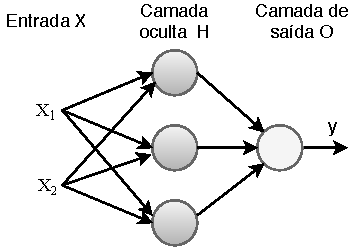
\includegraphics[width=0.4\textwidth]{figuras/feedforward.pdf}
	\caption[Rede \textit{feedforward} de 2 camadas]{Na rede \textit{feedforward} as informações fluem através das camadas. Não há conexões de retroalimentação nas quais as saídas do modelo sejam realimentadas. Adaptado de \cite{Goodfellow2016}.}
	\label{fig:feedforward}
\end{figure}


O teorema da aproximação universal \cite{hornik1989multilayer} estabelece que uma camada oculta é suficiente para uma rede \textit{feedfoward} aproximar qualquer função contínua em um subconjunto fechado e limitado de $R^{n}$ por uma rede neural e uma quantidade de erro diferente de zero \cite{Goodfellow2016}.

Seja $m_{0}$ o número de entradas de uma \acrshort{mlp} e M o número de neurônios na camada de saída. A relação de entrada-saída da rede define um mapeamento de um espaço de entrada euclidiano de dimensão $m_{0}$ para um espaço de saída euclidiano de dimensão M, que é infinitamente diferenciável desde que a função de ativação também tenha essa propriedade. Então o teorema diz:

\textit{Suponha que $\phi(.)$ seja uma função contínua não-constante, limitada e monotonamente crescente. Suponha que $I_{m_{0}}$ represente o hipercubo unitário $[0,1]^{m_{0}}$ de dimensão $m_{0}$. O espaço das funções contínuas em $I_{m_{0}}$ é representado por $C(I_{m_{0}})$. Então, dada qualquer função $f \in C(I_{m{0}})$ e $\epsilon>0$, existe um inteiro $m_{1}$ e conjuntos de constantes reais $\alpha_{i},\beta_{i}$ e $w_{ij}$, onde  $i = 1,...m_{1}$ e $j = 1, .., m_{0}$ tal que podemos definir:}

\begin{equation}
\label{eq:teorema_mlp}
\begin{aligned}
F(x_{1},..,x_{m_{0}}) = \sum_{i=1}^{m_{1}}\alpha_{i}\phi(\sum_{i=1}^{m_{0}}w_{ij}x_{j}+b_{i})
\end{aligned}
\end{equation}
\textit{como uma realização aproximada da função $f(.)$; isto é,}

\begin{equation}
\begin{aligned}
|F(x_{1},...,x_{m_{0}}) -f(x_{1},...,x_{m_{0}}) | < \epsilon
\end{aligned}
\end{equation}
\textit{para todo $x_{1},x_{2},..,x_{m_{0}}$ que se encontre no espaço de entrada}.

A equação apresentada em \ref{eq:teorema_mlp} representa uma rede \acrshort{mlp} com apenas uma camada oculta com $m_{1}$ neurônios. A ativação da camada oculta pode ser a função logística, uma vez que ela é não constante, limitada e monotonamente crescente. Os vetores \textbf{w} e \textbf{b} são os pesos e viés dos neurônios da camada oculta. A saída da rede é uma combinação linear das saídas dos neurônios ocultos, com \textbf{$\alpha$} definindo o vetor de pesos sinápticos da camada de saída \cite{Haykin}.  

Vale ressaltar que em novos trabalhos o teorema de aproximação universal foi provado para uma classe mais ampla de funções de ativação, como a \acrshort{relu} \cite{leshno1993multilayer}. Uma rede neural também pode aproximar qualquer mapeamento de função de qualquer espaço discreto dimensional finito para outro \cite{Goodfellow2016}.

O teorema da aproximação universal sintetizado pela Equação \ref{eq:teorema_mlp} generaliza as aproximações por série de Fourier \cite{Haykin}. Contudo, ele não define o mínimo número de neurônios  da camada oculta para cada $\epsilon$. Na pior das hipóteses, pode ser necessário um número exponencial de unidades ocultas (possivelmente uma unidade oculta correspondente a cada configuração de entrada que precise ser distinguida) \cite{Goodfellow2016}.
Além disso, o teorema também não diz se essa abordagem é ótima no sentido de tempo de de aprendizagem, facilidade de implementação e especialmente na generalização do modelo \cite{Haykin}. Na prática, as redes com mais de uma camada oculta se mostram mais concebíveis computacionalmente e generalizam melhor \cite{Goodfellow2016}.   

As principais considerações de arquitetura de uma \acrshort{rna} são a sua profundidade e o número de neurônios em cada camada. Redes mais profundas costumam usar  menos unidades por camada e menos parâmetros. Elas normalmente generalizam para o conjunto de testes, contudo são frequentemente difíceis de otimizar. A arquitetura de rede ideal para uma tarefa deve ser encontrada por meio de experimentação guiada pelo monitoramento do erro do conjunto de validação \cite{Goodfellow2016}.


\subsubsection{Rede Convolucional}

A \gls{rnc} é \textit{feedforward} apropriada para extrair atributos de imagens através da aplicação de convoluções bidimensionais em que os pesos dos filtros são aprendidos durante o treinamento. Ela é projetada especificamente para reconhecer formas bidimensionais com um alto grau de invariância quanto a translação, inclinação e outros modos de distorção. Isso significa que após aprender um certo padrão em uma posição específica de uma imagem a rede convolucional o reconhece em qualquer lugar da imagem \cite{Haykin}. 
A \gls{conv2d} é usada  em redes neurais para operar sobre mapas de características (estruturas  bidimensionais). Tais mapas estão organizados em pilhas formando tensores tridimensionais. Tensores podem ser interpretados como uma matriz multidimensional \cite{geron2017hands}, generalizando vetores e matrizes.  

Nesses tensores, a primeira e segunda dimensão são a altura e largura do mapa e a terceira dimensão é o número de canais ou, profundidade, ou ainda, o número de mapas recursos. A saída da convolução também é montada em tensores tridimensionais.
Os parâmetros para definir a operação de \acrshort{conv2d} são o passo (\textit{stride}), preenchimento (\textit{padding}), as dimensões espaciais do filtro e o número de canais de saída. O passo controla como o filtro se desloca pelos mapas. 
Através do preenchimento podemos adicionar um número apropriado de linhas e colunas em cada lado dos mapas. 
As duas principais configurações de preenchimento são as do tipo ``válida'' \textit(valid) e `mesma'' \textit{same}. Na primeira, não há preenchimento (somente locais válidos do mapa sofrem convolução pelo filtro), enquanto na segunda o preenchimento é feito de maneira a ter uma saída com a mesma largura e altura que a entrada \cite{FrancoisDeepLearning}. 
As dimensões espaciais do filtro se referem a sua altura e largura. O número de canais na saída da camada de convolução é igual à quantidade de filtros que foi escolhido para essa camada. O número de canais do filtro é sempre igual ao número de canais do tensor 3D de entrada. 

Matematicamente, a convolução de um tensor \textbf{I} com dimensões $H \times W \times 1$, por um filtro $K$($M \times N \times 1$), com passo 1 e  preenchimento válido, resulta no tensor \textbf{S} calculado segundo a equação a seguir. 

\begin{equation}
\label{eq:conv2d}
\begin{aligned}
S(i,j) = (I*K)(i,j)=  \sum_{m=0}^{M-1}\sum_{n=0}^{N-1}I(i+m,j+n)K(m,n) 
\end{aligned}
\end{equation}
onde $i \in [0,1,..., M-H+1]$ e $j \in [0,1,..., N-W+1]$. 

A Figura \ref{fig:con2d} ilustra a convolução 2D entre um mapa de recursos com um filtro $K = \begin{bmatrix}
1 &  0& 1\\ 
0 &  1& 0\\ 
1 &  0& 1
\end{bmatrix}$ .


\begin{figure}[h]
	\centering
	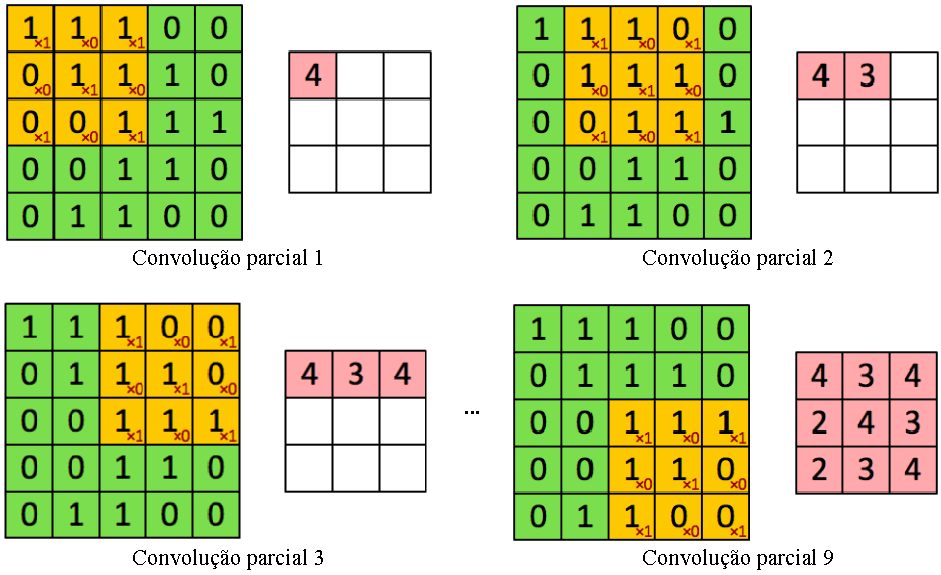
\includegraphics[width=0.6\textwidth]{figuras/conv2D.pdf}
	\caption[Convolução 2D em um mapa de recurso.]{Convolução de um tensor $5 \times 5 \times 1$, em verde, com um filtro $3 \times 3 \times 1$, em amarelo. À medida que o filtro se desloca pela entrada obtemos progressivamente um novo mapa de característica, em rosa, com dimensões $3 \times 3 \times 1$.  O filtro K se desloca 9 vezes, sempre executando uma operação de multiplicação ponto a ponto entre K e a parte P do mapa sobreposto pelo filtro. Em seguida, somamos todos os valores de K $\odot$ P para preencher o mapa de característica da saída \cite{sumit}.}
	\label{fig:con2d}
\end{figure}

Se a entrada for uma imagem com múltiplos canais, por exemplo, \acrshort{rgb}, então cada filtro da camada convolucional terá 3 canais.  Então, aplicamos a Equação \ref{eq:conv2d} em cada canal e todos os resultados são somados com o viés para fornecer uma saída. A Figura \ref{fig:con3d} ilustra uma etapa da convolução entre uma imagem \acrshort{rgb} com um filtro 3D para o cálculo do primeiro valor do mapa de característica. Uma função de ativação não-linear se aplica após a convolução.

\begin{figure}[h]
	\centering
	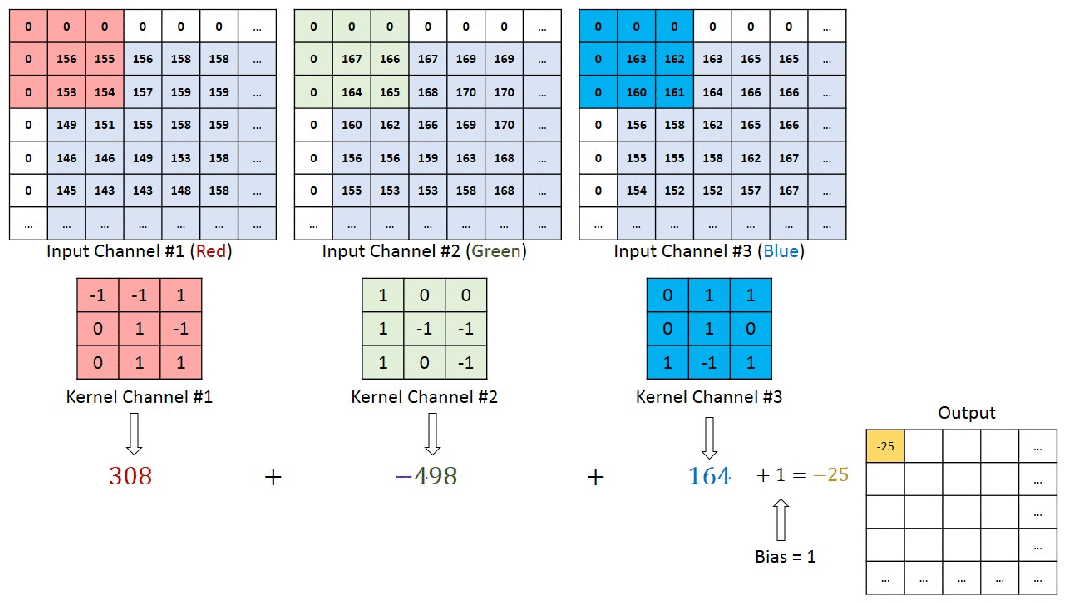
\includegraphics[width=0.9\textwidth]{figuras/conv3D.pdf}
	\caption[Convolução 2D em três mapa de recurso.]{Convolução de uma imagem  $5 \times 5 \times 3$, preenchido de zeros nas bordas, com um filtro K $3 \times 3 \times 1$. Para cada canal da imagem é feito uma convolução 2D com o respectivo canal do filtro. O resultado das convoluções são somados entre si e com o viés para fornecer a saída gradualmente.  O número de canais na saída é apenas 1 porque estamos utilizando 1 filtro \cite{sumit}.}
	\label{fig:con3d}
\end{figure}


Em uma rede convolucional, a unidade de processamento é representado por um filtro que recebe seus sinais de entrada de um campo receptivo local na camada anterior, aprendendo características locais \cite[272]{Haykin}. Os pesos dos filtros são os mesmos para cada mapa gerado. Esse compartilhamento de pesos é uma restrição estrutural que proporciona redução drástica do número de parâmetros livres em comparação com uma rede \acrshort{mlp} \cite[272]{Haykin}. 


%Em um rede convolucional é comum a operação de subamostragem após cada camada %convolucional. 
%A subamostragem pode ser feita calculando uma média local para cada região dos mapas %de características, reduzindo desta forma a resolução deles. Esta operação tem o efeito %de reduzir a sensibilidade da saída do mapa de características em relação a %deslocamentos e outras formas de distorção.


\subsection{Redes Recorrentes}

A \gls{rnr} \cite{rumelhart1986learning} é uma classe de redes neurais que incluem conexões de retroalimentação na sua arquitetura para processar dados sequenciais ou temporais. Para uma sequência $S = \{x_1,x_2,...,x_n\}$ a \acrshort{rnr} itera pelos seus elementos, mantendo um estado com informações relativas ao que foi visto até agora. Portanto, essa rede é projetada para ter memória \cite{FrancoisDeepLearning} e processar um conjunto de entrada arbitrariamente grande e de tamanho variável \cite{ketkar2017deep}.
A Figura \ref{fig:rnr} apresenta uma rede recorrente genérica em que a saída atual é uma função das saídas anteriores.  Essa formulação recorrente resulta no compartilhamento de parâmetros através do tempo essencial para a viabilidade e eficácia dessa rede \cite{Goodfellow2016}.

\begin{figure}[h]
	\centering
	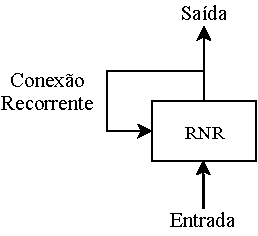
\includegraphics[width=0.3\textwidth]{figuras/rnn.pdf}
	\caption[Arquitetura RNR.]{Arquitetura básica para uma rede neural recorrente. As saídas anteriores são usadas na predição do estado atual. Adaptado de \cite{FrancoisDeepLearning}.}
	\label{fig:rnr}
\end{figure}

Podemos visualizar o compartilhamento dos pesos ao longo do tempo e o efeito dos resultados anteriores na saída atual pela próxima equação. 

\begin{equation}
\label{eq:memoria}
\begin{aligned}
\textbf{h}_{t} =  \phi( \textbf{x}_{t} \textbf{W} + \textbf{h}_{t-1} \textbf{U}) 
\end{aligned}
\end{equation}

Onde  $h_{t-1}$ e $h_{t}$ são os estados ocultos ou saídas da unidade recorrente no instante de tempo t-1 e t, respectivamente.  $x_{t}$ é a entrada da etapa  t da sequência, $\textbf{W}$ e $\textbf{U}$ são os vetores de pesos que multiplicam $x_{t}$ e $h_{t-1}$, respectivamente. Os pesos são compartilhados durante as iterações que compõem uma sequência de dados. A função de ativação está representada genericamente por $\phi \left( \odot \right)$. Devido ao ciclo da rede, o estado oculto, no instante t, depende de todos os estados ocultos obtidos anteriormente.  

O compartilhamento de parâmetros torna possível estender e aplicar o modelo a sequências de diferentes comprimentos, e identificar uma informação específica em qualquer posição dentro da sequência \cite{Goodfellow2016}. 
Para treinar uma RNR é preciso executar o algoritmo de retropropagação ao longo das etapas para cada sequência. Isso requer desenrolar a RNR em uma rede profunda. O treinamento de uma rede neural profunda pode sofrer com lentidão e problemas de gradientes que tendem a zero ou a valores muito elevados. A solução mais simples e comum para esse problema é desenrolar a RNR apenas em um número limitado de etapas durante o treinamento. Isso é chamado de retropropagação truncada ao longo do tempo \cite{geron2017hands}.

Atualmente, um dos modelos de sequências mais eficazes usados em aplicações práticas é a \gls{lstm} \cite{lstm}. A sua arquitetura favorece a rápida convergência e detecção de dependências de longo prazo nos dados \cite{geron2017hands}.
Essas redes contém  têm ``células LSTM'' que possuem uma recorrência interna além da recorrência externa. Veja a Figura \ref{fig:lstm_time} para observar essas duas recorrências. Cada célula possui as mesmas entradas e saídas que uma rede recorrente comum, mas contém mais parâmetros e um sistema de unidades de controle que coordena o fluxo de informações.  A formulação matemática da \acrshort{lstm} possui 4 camadas de rede neural sendo 3 delas unidades de controle ou portas. 

\begin{equation}
\label{eq:lstm}
\begin{aligned}
\textbf{i}_t &= \sigma_{i}(\textbf{W}_i\textbf{x}_t + \textbf{U}_i\textbf{h}_{t-1} + \textbf{b}_i) \\
\textbf{f}_t &= \sigma_{g}(\textbf{W}_f\textbf{x}_t + \textbf{U}_f\textbf{h}_{t-1} + \textbf{b}_f) \\
\textbf{o}_t &= \sigma_{o}(\textbf{W}_o\textbf{x}_t + \textbf{U}_o\textbf{h}_{t-1} + \textbf{b}_o) \\   
\textbf{c}'_t &= tanh(\textbf{W}_c\textbf{x}_t + \textbf{U}_c\textbf{h}_{t-1} + \textbf{b}_c) \\
\textbf{c}_t &= \textbf{f}_t \odot \textbf{c}_{t-1} + \textbf{i}_t \odot \textbf{c}'_t \\
\textbf{h}_t & = \textbf{o}_t \odot \tanh(\textbf{c}_t)  
\end{aligned}
\end{equation}
Onde, $\textbf{x}_t$ é a entrada atual da sequência. As variáveis $\textbf{W}$, $\textbf{U}$ e $\textbf{b}$  são as matrizes de pesos e viés aprendidas por cada camada.  O vetor $\textbf{i}_{t}$ é a porta de entrada que nos diz quais novas informações vamos armazenar no estado da célula, $\textbf{c}_{t}$. 
A porta do esquecimento, $\textbf{f}_{t}$, controla quais informações serão ``esquecidas'' do estado da célula anterior, $\textbf{c}_{t-1}$. A porta de saída $\textbf{o}_{t}$ é usada para fornecer a ativação para a saída, $\textbf{h}_{t}$. O vetor $\textbf{c}'_{t}$ é o estado da célula candidata e $\textbf{c}_{t}$ é o estado de célula atual.  Este último é o termo que contém a ``memória'' de longo prazo da \acrshort{lstm}. Nessa equação, o símbolo $\odot$ significa multiplicação ponto a ponto entre dois vetores. O cálculo do estado de célula é uma função recursiva que ocorre no interior da célula. Por fim, a saída é um o vetor $\textbf{h}_{t}$.
A função logística é adotada na ativação das 3 portas.  Dessa forma, as portas podem inibir uma informação na medida que seus elementos sejam próximos de zero (saturação inferior) ou mantê-la se os seus elementos são próximos a um (saturação superior). A lista a seguir detalha as variáveis da \acrshort{lstm} quando o vetor $\textbf{x}_t$ tem tamanho $d$ e escolhemos $h$ unidades ocultas.    


\begin{enumerate}
	\item $\textbf{x}_t \in \mathbb{R}^{d}$
	\item $\textbf{f}_t,\textbf{i}_t,\textbf{o}_t,\textbf{h}_t,\textbf{c}'_t,\textbf{c}_t \in \mathbb{R}^{h}$ 
	\item $\textbf{W} \in \mathbb{R}^{h \times d} $
	\item $\textbf{U} \in \mathbb{R}^{h \times h}$
	\item $\textbf{b} \in \mathbb{R}^{h}$
\end{enumerate}

\begin{figure}[h]
	\centering
	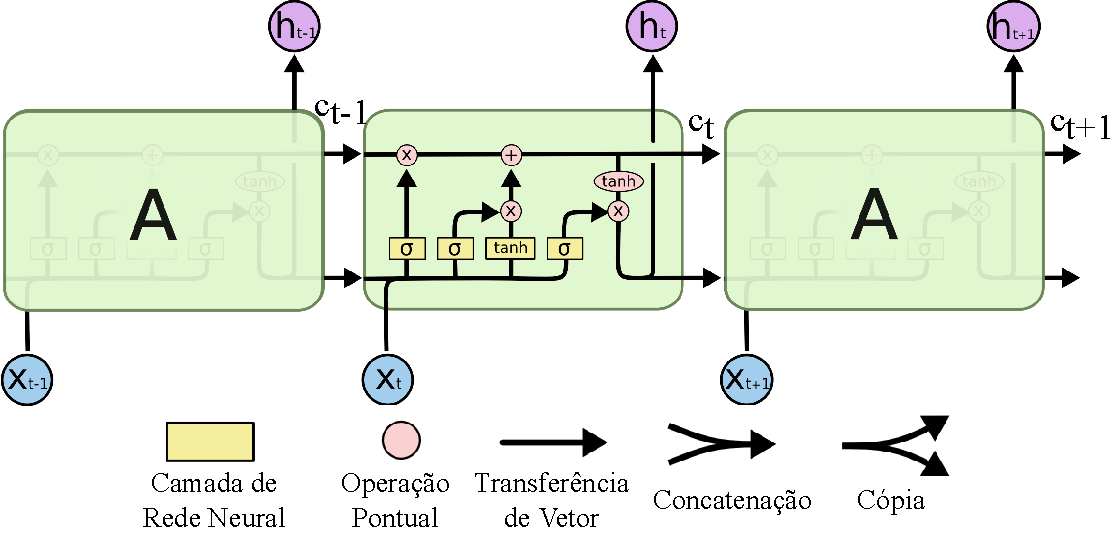
\includegraphics[width=0.7\textwidth]{figuras/lstm_no_tempo.pdf}
	\caption[Célula \acrshort{lstm} no tempo]{Célula \acrshort{lstm} desenrolada no tempo. O estado de célula $\textbf{c}_{t}$ e estado oculto $\textbf{h}_{t}$ são usados para realimentar a célula a cada etapa de tempo. O primeiro é calculado em um ciclo interno enquanto o segundo é obtido por recorrência externa à \acrshort{lstm}. Adaptado de \cite{Olah}.}
	\label{fig:lstm_time}
\end{figure}

A formulação da \acrshort{lstm} apresentada aqui é também denominada por \gls{fc-lstm}.

A sua principal desvantagem, no tratamento de dados espaço-temporais, é o fato que não leva em consideração uma correlação espacial devido ao uso de conexões completas nas operações internas.  
Para superar esse problema, defini-se a \gls{conv2dlstm} \cite{xingjian2015convolutional,FullResolution2017Toderici} na qual todas as entradas($x_1,..., x_t$), estados de células ($c_1,..., c_t$), estados ocultos($h_1,..., h_t$) e portas($i_t$, $f_t$, $o_t$) são tensores 3D cujas duas últimas dimensões são dimensões espaciais (linhas e colunas). Isso pode ser alcançado usando um operador de convolução nas transições de estado para estado e de entrada para estado. As principais equações do \acrshort{conv2dlstm} são mostradas abaixo, onde '*' denota o operador de convolução

\begin{equation}
\label{eq:conlstm}
\begin{aligned}
\textbf{i}_t &= \sigma_{i}(\textbf{W}_i*\textbf{x}_t + \textbf{U}_i*\textbf{h}_{t-1} + \textbf{b}_i) \\
\textbf{f}_t &= \sigma_{g}(\textbf{W}_f*\textbf{x}_t + \textbf{U}_f*\textbf{h}_{t-1} + \textbf{b}_f) \\
\textbf{o}_t &= \sigma_{o}(\textbf{W}_o*\textbf{x}_t + \textbf{U}_o*\textbf{h}_{t-1} + \textbf{b}_o) \\   
\textbf{c}'_t &= tanh(\textbf{W}_c*\textbf{x}_t + \textbf{U}_c*\textbf{h}_{t-1} + \textbf{b}_c) \\
\textbf{c}_t &= \textbf{f}_t \odot \textbf{c}_{t-1} + \textbf{i}_t \odot \textbf{c}'_t \\
\textbf{h}_t & = \textbf{o}_t \odot \tanh(\textbf{c}_t)  
\end{aligned}
\end{equation}

%Para obter uma melhor imagem das entradas e estados, podemos imaginá-las como vetores em pé em uma grade espacial. O ConvLSTM determina o estado futuro de uma determinada célula na grade pelas entradas e estados passados de seus vizinhos locais.

\subsection{Autocodificadores}

%O \textit{autoencoder}  é uma rede neural treinada  para tentar reconstruir os dados de entrada na saída.

O \gls{ac}, é uma rede neural que mapeia a entrada $x$ para um espaço vetorial latente, $z$, por meio de um módulo de codificador $E$, e depois a decodifica de volta para uma saída $x'$ com as mesmas dimensões da entrada original, por meio de um módulo de decodificador $D$ \cite{FrancoisDeepLearning}. Esse processo é resumido por: 

\begin{equation}
\begin{aligned}[alignment]
z &= E(x)\\ 
x' &= D(z)	
\end{aligned}
\end{equation}

Nessa rede, o processo de aprendizagem visa minimizar uma função de perdas:
\begin{equation}
L = d(x,D(E(x)))
\end{equation}

Onde $d$ é uma função de perda que penaliza $D(E(x))$  por ser diferente de $x$. Na prática, os \acrshort{ac}es clássicos não levam a espaços latentes particularmente úteis ou bem estruturados \cite{FrancoisDeepLearning}. 

%A rede pode ser vista como consistindo de duas partes: uma função de codificação, $\textbf{z} = E(\textbf{x})$ e um decodificador que produz a reconstrução $\textbf{f} = D(\textbf{z})$ \cite{Goodfellow2016}. 


Um \acrshort{ac} é dito incompleto quando a dimensão de saída do codificador é menor que a dimensão de entrada \cite{Goodfellow2016}. Nesse caso, o codificador realiza sucessivas transformações de filtragens e reduções na dimensionalidade dos dados de entrada, em um processo chamado de subamostragem, do inglês (\textit{downsampling}), e produz o vetor latente. O vetor latente segue para o decodificador que irá aumentar a dimensionalidade dos dados na etapa de superamostragem (\textit{upsampling}) e produz uma versão aproximada dos dados de entrada. Aprender uma representação incompleta força o \textit{autoencoder}  a capturar os recursos mais destacados dos dados de treinamento \cite{Goodfellow2016}. 


%Esses dois elementos são treinados de ponta a ponta, mas durante a implantação, o codificador e o decodificador são normalmente usados independentemente.




%- um tipo de rede que visa codificar uma entrada para um espaço latente de baixa dimensão e depois decodificá-la de volta -
% Em seguida, ele é treinado usando como dados de destino as mesmas imagens que as imagens de entrada, o que significa que o \textit{autoencoder}  aprende a reconstruir as entradas originais \cite{FrancoisDeepLearning}.

%Uma maneira de obter recursos úteis do codificador automático é restringir h a ter uma dimensão menor que x.

\subsubsection{Autocodificador Esparso}

Um \acrshort{ac} esparso possui um critério de treinamento que envolve uma penalidade de esparsidade $\Omega(z)$ na camada da representação do vetor latente, além do erro de reconstrução \cite{Goodfellow2016}:

\begin{equation}
\label{eq:loss_sparse}
\begin{aligned}
L = d(x,D(E(x))) + \Omega(z) 
\end{aligned}
\end{equation}

Se impusermos uma restrição de esparsidade às unidades do latente, o codificador automático descobrirá uma estrutura interessante nos dados, mesmo que o número de unidades ocultas seja grande \cite{ng2011sparse}. 
Para uma função de ativação logística, considera-se um neurônio como sendo ``ativo'' se seu valor de saída for próximo de 1 ou como ``inativo'' se seu valor de saída for próximo de 0. Sendo $z_j$ a ativação de uma unidade do vetor latente ${z}$ para uma entrada específica $x_m$ podemos definir uma média da ativação dessa unidade para um conjunto com $M$ exemplos de treinamento:

\begin{equation}
\hat{\rho}_{j} = \frac{1}{M}\sum_{i=1}^M z_j
\end{equation}

Em um \acrshort{ac} esparso desejamos obter neurônios inativos na maioria das vezes, isto é, queremos impor a restrição:

\begin{equation}
\hat{\rho}_{j} = \rho
\end{equation}

onde ${\rho}$ é um parâmetro de esparsidade, normalmente um valor pequeno próximo a zero. 
Então, escolhemos uma função que penaliza $\hat{\rho}_{j}$ por ser diferente de ${\rho}$. Uma opção, é usar a divergência de 
de Kullback-leibler (KL) \cite{kullback1951information} entre duas variáveis aleatórias de Bernoulli com médias ${\rho}$ e $\hat{\rho}_{j}$: \cite{ng2011sparse}.  

\begin{equation}
D_{KL}(\rho||\hat{\rho}_{j}) = \sum_{j=1}^{h}\rho \log \frac{\rho}{\hat{\rho}_{j}} +(1-\rho)\log \frac{1- \rho}{1-\hat{\rho}_j}
\end{equation}

Aqui, $h$ é o número de elementos do latente.  A divergência KL é uma função padrão para medir a diferença entre duas distribuições diferentes. Ela tem a propriedade que $D_{KL}(\rho||\hat{\rho}_{j}) = 0$ se $\rho = \hat{\rho}_{j}$ e, caso contrário, aumenta monotonicamente à medida que $\hat{\rho}_{j}$ diverge de $\rho$ \cite{kullback1951information}. Então podemos reescrever a Equação \ref{eq:loss_sparse} como:

\begin{equation}
\label{eq:loss_sparse2}
\begin{aligned}
L = d({x},D(E({x}))) + \lambda \sum_{j=1}^{s_2} D_{KL}(\rho||\hat{\rho}_{j}) 
\end{aligned}
\end{equation}
Onde $\lambda$ controla o peso do termo de penalidade de esparsidade. Geralmente, restringimos o latente a ser de baixa dimensão e esparso para que o codificador atue para compactar os dados de entrada em menos bits de informação \cite{FrancoisDeepLearning}.

%Para satisfazer essa restrição, as ativações da unidade oculta devem estar próximas de 0.

%Um codificador automático que foi regularizado para ser esparso deve responder a recursos estatísticos exclusivos do conjunto de dados em que foi treinado, em vez de simplesmente atuar como uma função de identidade. Dessa forma, o treinamento para executar a tarefa de cópia com uma penalidade de escassez pode produzir um modelo que aprendeu recursos úteis como subproduto.
%Podemos pensar na penalidade $\Omega(h)$ simplesmente como um termo regularizador adicionado a uma rede feedforward cuja tarefa principal é copiar a entrada na saída 
%Ao contrário de outros regularizadores, como a redução de peso, não há uma interpretação bayesiana direta para esse regularizador. 



%Ao impor várias restrições ao código (a saída do codificador), você pode fazer com que o \textit{autoencoder}  aprenda representações latentes mais ou menos interessantes dos dados. 


\subsubsection{Autocodificador Variacional}


O \gls{vae} \cite{kingma2013auto,rezende2014stochastic} é um modelo generativo profundo capaz de aprender representações latentes não supervisionadas de dados \cite{klys2018learning}.
Um \acrshort{vae} transforma uma entrada em parâmetros de uma distribuição estatística. Isso significa assumir que a entrada foi gerada por um processo estatístico e que a aleatoriedade desse processo deve ser levada em consideração durante a codificação e decodificação \cite{FrancoisDeepLearning}.

Seja $X = \{x^i\}_{i=1}^N$ uma base de dados consistindo de $N$ amostras independentes e identicamente distribuídas, gerada de uma variável aleatória $x$. Um \acrshort{ac} opera com dois mapeamentos, o codificador opera $Enc_{\phi}:X \rightarrow Z$ e o decodificador $Dec_{\theta}:Z \rightarrow X$, onde $Z$ é o espaço latente. No caso do \acrshort{vae}, ambos os mapeamentos são probabilísticos e uma distribuição fixa a \textit{prior} $p(z)$ sobre $Z$ é assumida. Como a distribuição de $x$ também é fixa (distribuição de dados real $q(x)$), os mapeamentos $Enc_{\phi}$ e  $Dec_{\theta}$ induzem distribuições conjuntas $q(x,z) = q_{\phi}(z|x)q(x)$ e $p(x,z) = p_{\theta}(x|z)p(z)$, respectivamente (omitindo a dependência com os parâmetros $\theta$ e $\phi$) \cite{rolinek2019variational}. O objetivo idealizado do \acrshort{vae} é obter a função de verossimilhança logarítmica (\textit{log-likelihood}) marginalizada:


\begin{equation}
\sum_{i=1}^N \log (p(x^i))
\end{equation}

Entretanto, esse objetivo não é tratável e é aproximado pelo limite inferior da evidência (ELBO) \cite{kingma2013auto}. Para um $x_i$ fixo, o logarítmico de verossimilhança $\log p(x^i)$ tem o limite inferior dado por $\mathcal{L}(q)$ conforme a seguinte equação:

\begin{equation}
\label{elbo}
\mathcal{L}(q) = \mathbb{E}_{z \sim q(z|x^i)} \log p(x_i|z) - D_{KL}(q(z|x^i)||p(z)) \leq \log p(x^i)
\end{equation}

onde o primeiro termo corresponde à perda de reconstrução e o segundo à divergência KL entre a representação latente $q(z|x_i)$ e a distribuição a \textit{prior} $p(z)$.
Por fim, $p(z)$ é definido como uma distribuição gaussiana multidimensional com média zero: $\mathcal{N}$(0, $\mathcal{I}$) onde $\mathcal{I}$ é a matriz identidade. O codificador também assume o formato de uma distribuição gaussiana dada por:

\begin{equation}
Enc_{\theta}(x) \sim q_{\phi}(z|x) = \mathcal{N}(\mu_{\phi}(x), diag\ \ \sigma_{\phi}^2(x))
\end{equation}
%The important property here is that pθ(x|z) can be efficiently computed
%Uma variante, o $\beta$-VAE [17], introduz uma ponderação $\beta$ no termo KL para regular o trade-off entre reconstrução (primeiro termo) e a proximidade com $p(z)$. 
onde $\mu_{\phi}$ e $\sigma_{\phi}$ são mapeamentos determinísticos que dependem dos parâmetros $\phi$. A matriz de covariância é aplicada para ser diagonal. Os parâmetros de geração e inferência, $\theta$ e  $\phi$, são treinados em conjunto pela maximização de $\mathcal{L}$, onde usamos o truque de reparametrização para aplicar a descida estocástica do gradiente através das variáveis latentes gaussianas \cite{sonderby2016ladder}. Além disso, todas as expectativas na Equação \ref{elbo} podem ser aproximadas pela amostragem de Monte Carlo \cite{Goodfellow2016}.
Uma vez concluído o treinamento, a distribuição a \textit{posterior} aproximado $q_{\phi}(z|x)$ funciona como um codificador.



%Tomando  $\mathcal{X}$ como pontos no conjunto de dados, considere um vetor de variáveis latente $z$ em um $\mathcal{Z}$ de alta dimensão facilmente amostrado por um PDF $P(z)$ definido de $\mathcal{Z}$. 
%Então, é possível considerar uma família de funções $f(z; \theta)$  parametrizada por $\theta$ em um espaço $\Theta$ em que $f:\mathcal{Z} \times \Theta \rightarrow \mathcal{X}$. Como $z$ é aleatório, $f(z;\theta)$  é uma variável aleatória em $\mathcal{X}$. Desejamos otimizar $\theta$ de modo que possamos amostrar $z$ de $P(z)$ e, com alta probabilidade, $f(z;\theta)$ será como os X's em nosso conjunto de dados.


%\cite {TutorialVAE2016Doersch}.

%Matematicamente, a seguinte equação precisa ser maximizada:
%\begin{equation}%
%	P(X) = \int P(X|z; \theta)P(z)dz
%\end{equation}

%onde $P(X|z; \theta)$ representa $f(z;\theta)$. Para definir as variáveis latente $z$, os \acrshort{vae} assumem que não há uma interpretação simples das dimensões de $z$ e afirme que amostras de $z$ podem ser extraídas de $\mathcal{N}(0,I)$, onde $I$ é a matriz de identidade.Além disso, a integral acima pode ser calculada através de um grande número de valores z $\{z_1,...,z_n\} $com $P(x) \approx \frac{1}{n} \sum_{i}^{} P(X|z_i)$. 


%Para gerar uma amostra do modelo, o \acrshort{vae} primeiro extrai uma amostra $z$ da distribuição de código $p_modelo(z)$. A amostra é então executada através de uma rede geradora diferenciável $g(z)$. Finalmente, $x$ é amostrado de uma distribuição $p_{modeolo}(x;g(z)) = p_{modelo}(x|z)$. Entretanto, durante o treinamento, a rede de inferência aproximada (ou codificador) $q(z|x)$ é usada para obter $z$ e $p_{modelo}(x|z)$ é então vista como um decodificador rede.



%O \acrshort{vae} usa os parâmetros de média e variância para amostrar aleatoriamente um elemento da distribuição e decodifica esse elemento de volta à entrada original. A estocástica deste processo melhora a robustez e força o espaço latente a codificar representações significativas em todos os lugares: todo ponto amostrado no espaço latente é decodificado para uma saída válida \cite{FrancoisDeepLearning}.

%O principal insight por trás dos autoencodificadores variacionais é que eles podem ser treinados maximizando o limite inferior variacional $L(q)$ associado ao ponto de dados x.





%Em termos técnicos, veja como um \acrshort{vae} funciona:
%Um módulo codificador transforma as amostras de entrada input\_img em dois parâmetros em um espaço latente de representações, z\_mean e z\_ log\_variance.
%Você experimenta aleatoriamente um ponto z da distribuição normal latente que se supõe gerar a imagem de entrada, via z = z\_mean + exp (z\_log\_variance) * epsilon, em que epsilon é um tensor aleatório de pequenos valores.
%Um módulo decodificador mapeia esse ponto no espaço latente de volta à imagem de entrada original.Como o epsilon é aleatório, o processo garante que todos os pontos próximos ao local latente em que você codificou input\_img (z-mean) possam ser decodificados para algo semelhante a input\_img, forçando o espaço latente a ser continuamente significativo. Quaisquer dois pontos próximos no espaço latente decodificarão para imagens altamente semelhantes. A continuidade, combinada com a baixa dimensionalidade do espaço latente, força todas as direções no espaço latente a codificar um eixo significativo de variação dos dados, tornando o espaço latente muito estruturado e, portanto, altamente adequado para manipulação por vetores conceituais.

%Os parâmetros de um \acrshort{vae} são treinados por meio de duas funções de perda: uma perda de reconstrução que força as amostras decodificadas a corresponderem às entradas iniciais e uma perda de regularização que ajuda a aprender espaços latentes bem formados e reduzir a adaptação excessiva aos dados de treinamento. Vamos analisar rapidamente uma implementação Keras de um VAE. Esquematicamente, é assim:




%Na equação 20.76, reconhecemos o primeiro termo como a probabilidade logarítmica conjunta das variáveis ​​visíveis e ocultas sob o posterior aproximado sobre as variáveis ​​latentes (assim como no EM, exceto que usamos um posterior aproximado, e não o exato). Reconhecemos também um segundo termo, a entropia do posterior aproximado. Quando q é escolhido para ser uma distribuição gaussiana, com ruído adicionado a um valor médio previsto, maximizar esse termo de entropia incentiva o aumento do desvio padrão desse ruído. De maneira mais geral, esse termo de entropia encoraja a variação posterior a colocar uma massa de alta probabilidade em muitos valores de z que poderiam ter gerado x, em vez de entrar em colapso para uma estimativa pontual do valor mais provável. Na equação 20.77, reconhecemos o primeiro termo como a probabilidade de log de reconstrução encontrada em outros autoencodificadores. O segundo termo tenta fazer com que a distribuição posterior aproximada q (z | x) e o modelo anterior p modelo (z) se aproximem.

%As abordagens tradicionais para inferência variacional e aprendizado inferem q por meio de um algoritmo de otimização, tipicamente iteradas equações de ponto fixo (seção 19.4). Essas abordagens são lentas e geralmente exigem a capacidade de calcular o modelo E z∼q log p (z, x) de forma fechada. A idéia principal por trás do \textit{autoencoder}  variacional é treinar um codificador paramétrico (também chamado de rede de inferência ou modelo de reconhecimento) que produz os parâmetros de q. Contanto que z seja uma variável contínua, podemos então propagar novamente através de amostras de z extraídas de q (z | x) = q (z; f (x; θ)) para obter um gradiente em relação a θ. O aprendizado então consiste apenas em maximizar L com relação aos parâmetros do codificador e decodificador. Todas as expectativas em L podem ser aproximadas pela amostragem de Monte Carlo.
%A aprendizagem então consiste apenas em maximizar $\mathcal{L}$ com relação aos parâmetros do codificador e decodificador. 


\section{Compressão de dados}
Nessa seção, apresentamos o problema da compressão de dados e o papel desempenhado pelo par \gls{codec}. Além disso, também é tratado, superficialmente, um desenvolvimento probabilístico proposto por Shanon para mensurar a informação e estabelecer, dentro das suas hipóteses, um valor mínimo ótimo de taxa de compressão sem perdas.

A compressão de dados compreende o processo de reduzir o espaço em memória ocupado por dados que representam uma dada informação. Os dados são os meios pelos quais as informações são transmitidas \cite{gonzalez2009processamento}. Sejam $b$ e $b’$ o número de bits de duas representações das mesmas informações, a taxa de compressão $C$ e a redundância relativa de dados, $Rd$, da representação $b$ em relação a $b'$ são:

\begin{equation}
\label{eq:compressao}
\begin{aligned}
C &= \frac{b}{b'} \\
Rd &= 1 - \frac{1}{C}
\end{aligned}
\end{equation}

Considerando que a informação representada pelos $b$ bits contém $s$ símbolos, então, defini-se a taxa dessa representação ou número médio de bits como $R = \frac{b}{s}$ bits por símbolo (bps).   

O codificador é o algoritmo utilizado para explorar as redundâncias na informação e gerar um conjunto de dados comprimidos. O algoritmo do decodificador realiza o processo de reconstrução dos dados. Ele toma os dados comprimidos e tenta recuperar os dados originais que representam a informação. Esse processo está ilustrada na Figura \ref{fig:codec}.


\begin{figure}[h]
	\centering
	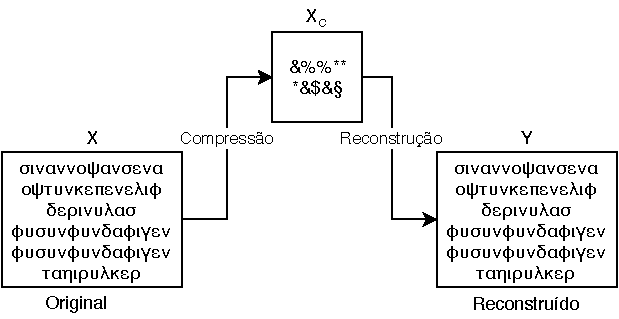
\includegraphics[width=0.6\textwidth]{figuras/codec.pdf}
	\caption[Compressão e reconstrução sem perdas.]{O algoritmo de compressão (codificador) recebe uma entrada X e gera uma representação X$_c$ que requer menos bits. O algoritmo de reconstrução (decodificador) opera na representação compactada X$_c$ para gerar a reconstrução Y. Adaptado de \cite{sayood2017introduction}.}
	\label{fig:codec}
\end{figure}


Esses dois algoritmos formam o \acrshort{codec}. Ele pode ser projetado para tratar com categorias de informações específicas que incluem, por exemplo, imagens, áudios e vídeos. 

%Embora seja verdade que as capacidades de armazenamento e transmissão estão aumentando constantemente com novas inovações tecnológicas, como um corolário da Primeira Lei de Parkinson, parece que a necessidade de armazenamento em massa e transmissão aumenta pelo menos duas vezes mais rápido que as capacidades de armazenamento e transmissão \cite{sayood2017introduction}.

A compressão pode ser com perdas e sem perdas. No primeiro tipo o codificador introduz restrições que faz o decodificador recuperar dados que aproximam a representação da informação original ao passo que na compressão sem perdas os dados recuperados são exatamente iguais aos originais \cite{sayood2017introduction}. 
%No geral, as compressões com perdas apresentam a vantagem de alcançar taxas de compressão maiores que a compressão sem perdas ao custo de perder parte da informação. 

\subsection{Medidas de informação}

%A teoria da informação proporciona a estrutura conceitual matemática para mensurar a quantidade mínima de %dados para representar uma informação. A teoria da informação fornece as ferramentas necessárias para representar e manipular informações de forma direta e quantitativa. 

A geração da informação pode ser modelada como um processo probabilístico medido de maneira intuitiva. Conforme essa suposição, dizemos que um evento aleatório $E$ que ocorra com probabilidade $P(E)$ contém $I(E)$ unidades de informação dada por \cite{marques1999processamento}:

\begin{equation}
\begin{aligned}
I(E) = log_{b}\frac{1}{P(E)} = - \log (P(E)) 
\end{aligned}
\end{equation}

onde a base $b$ do logaritmo define a unidade utilizada para medir as informações. Se a base 2 for selecionada, a unidade de informação é o bit. $I(E)$ também é denominado de auto-informação. Se tivermos um conjunto de eventos independentes $A_i$ provenientes de algum experimento $S$, tais que:

\begin{equation}
\bigcup A_i = S 
\end{equation}

sendo $S$ o espaço amostral, então a auto-informação média associada ao experimento aleatório é fornecida por:

\begin{equation}
H(x) = -\sum P(A_i)\log_b(P(A_i))
\end{equation}

Essa quantidade é chamada entropia associada ao	experimento. Se o experimento é uma fonte que gera os símbolos $A_i$ de um conjunto $\mathcal{A}$ denominado alfabeto da fonte, a entropia é uma medida do número médio de símbolos binários necessários para codificar a saída da fonte  \cite{sayood2017introduction}. Ademais, essa quantidade é a mínima necessária para que qualquer método de compressão codifique essa fonte sem perdas.

Contudo, se o conjunto de eventos gerados são dependentes devemos considerar tais dependências para pode estimar de forma mais precisa a entropia real da fonte. 
Uma possibilidade para realizar essa estimação é observar distribuições conjuntas de sequências de símbolos cada vez mais longas \cite{sayood2017introduction}. Para uma sequência de comprimento $n$, podemos definir a entropia de ordem $n$ que se aproxima da entropia real da fonte à medida que $n$ aumente. 


%\begin{equation}
%\begin{aligned}
%H_n =  - \dfrac{1}{n}\sum_{i_1=1}^{m}\sum_{i_2=1}^{m} … \sum_{i_n=1}^{m}P(X_1 = i_1) P(X_2 = i_2).. P(X_n =i_n) \\ \times log_b(P(X_1 = i_1)log_b(P(X_1 = i_1)...log_b(P(X_n = i_n)) 
%\end{aligned}
%\end{equation}

%Dessa forma, capturamos as dependências do elementos observando as distribuições conjuntas de sequências cada vez mais longas geradas pela fonte. Quando n tende ao infinito $H_n$ converge para a entropia real da fonte. 

\section{Imagens}


Uma imagem pode ser definida como uma função bidimensional, $f(x,y)$, em que $x$ e $y$ são coordenadas espaciais (plano), e a amplitude de f em qualquer par de coordenadas $(x, y)$ é chamada de intensidade ou valor do \textit{pixel} nesse ponto \cite{gonzalez2009processamento}. Em uma imagem digital os valores de $x$,$y$ e $f$ são discretos e finitos. 
Uma imagem monocromática requer apenas um número para indicar a intensidade de cada amostra espacial. As imagens coloridas, por outro lado, exigem pelo menos três números por posição de pixel para representar com precisão as cores \cite{richardson2010h}.

\subsection{Espaço de Cores}

As três características normalmente utilizadas para distinguir as cores entre si são:
brilho ou luminância (\textit{brightness}), matiz (\textit{hue}) e saturação (\textit{saturation}). O brilho representa a noção de intensidade luminosa da radiação, o matiz é uma propriedade associada ao comprimento de
onda predominante na combinação das várias ondas visíveis, enquanto a saturação expressa a pureza do matiz ou o grau de mistura do matiz original com a luz branca \cite{marques1999processamento}. O matiz e a saturação são denominados conjuntamente de cromaticidade.
O método escolhido para representar brilho e cor é descrito como um espaço de cores \cite{richardson2010h}. O objetivo dos modelos de cores é permitir a especificação de cores em um formato padronizado e aceito por todos \cite{gonzalez2009processamento}. 

\subsubsection{RGB}
No espaço de cores \gls{rgb}, a imagem colorida é representada com três números que indicam as proporções relativas de vermelho, verde e azul, as três cores primárias aditivas da luz \cite{richardson2010h}. Combinar vermelho, verde e azul em proporções variadas pode criar qualquer cor. O modelo pode ser visto como um cubo onde três de seus vértices são as cores primárias, o vértice junto à origem é o preto e o mais afastado da origem corresponde à cor branca \cite{gonzalez2009processamento}. 

\begin{figure}[h]
	\centering
	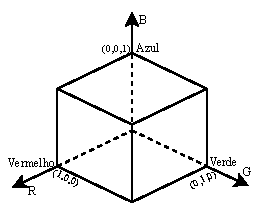
\includegraphics[width=0.4\textwidth]{figuras/rgb.pdf}
	\caption[Espaço tridimensional de cores RGB.]{Espaço de cores RGB representado em um cubo. Adaptado de \cite{gonzalez2009processamento}.}
	\label{fig:rgb}
\end{figure}

\subsubsection{YCbCr}

O sistema visual humano é menos sensível à cor do que à luminância (Y). No espaço de cores \acrshort{rgb}, as três cores são igualmente importantes e, geralmente, armazenadas na mesma resolução. Contudo, é possível representar uma imagem colorida com mais eficiência, separando a luminância das informações de cores e representando Y com uma resolução maior que a cor \cite{richardson2010h}. O componente de luminância é calculado como uma média R, G e B ponderada pelos pesos $k_r$, $k_g$ e $k_b$, respectivamente.

\begin{equation}
\begin{aligned}
Y = k_rR + k_gG + k_bB 
\end{aligned}
\end{equation}

Cada componente de crominância é a diferença entre R, G ou B e Y.

\begin{equation}
\begin{aligned}
Cr &= R - Y \\
Cb &= B - Y \\
Cg &= G - Y
\end{aligned}
\end{equation}



%A maioria das imagens são representadas com 8 bits, isto é, com 256 valores discretos para a intensidade. Em uma imagem colorida representada no espaço de cores RGB \textit(Red,Green e Blue), cada pixel tem 24 bits de resolução de intensidade, 8 bits para cada imagem componente de cor: vermelha, verde e azul \cite{gonzalez2009processamento}.



\subsection{Compressão de Imagens}

%A tarefa de compressão de imagens é importante para promover reduções no espaço de memória ocupada para armazená-las e na largura de banda para transmitir os dados pela redes de comunicações. Da teoria de telecomunicações, sabe-se que se a taxa de transmissão de um sinal é reduzida então a largura de banda requisitada para transmitir os dados também será menor.

No contexto da compressão digital de imagens os três principais tipos de redundância de dados que podem ser identificados e explorados são \cite{gonzalez2009processamento}:
\begin{enumerate}
	\item Redundância de codificação. Os códigos de 8 bits utilizados para representar as intensidades na maioria dos arranjos de intensidade	2-D contêm mais bits do que o necessário para representar as intensidades.
	\item Redundância espacial. Como os \textit{pixels} da
	maioria dos arranjos de intensidade 2-D são correlacionados no espaço (isto é, cada pixel é similar aos \textit{pixels} vizinhos ou dependente deles), as informações são desnecessariamente replicadas nas representações dos \textit{pixels} correlacionados.
	\item Informações irrelevantes. A maioria dos arranjos de intensidade 2-D contém informações ignoradas pelo sistema visual humano e/ou irrelevantes para a utilização pretendida da imagem. 
\end{enumerate}


\subsubsection{JPEG}

O JPEG é o acrônimo de \textit{Joint Photographic Experts Group}. Foi concebido por um esforço conjunto do \gls{ccitt} (agora \gls{itu}) e da \gls{iso}. Ele é um dos padrões mais conhecidos para compactação de imagem com perdas, amplamente usado na \textit{Web} e em máquinas fotográficas \cite{sayood2017introduction}. 
As principais etapas desse \acrshort{codec} estão descritas a seguir. 
\begin{enumerate}
	\item A primeira etapa consiste em transformar uma imagem colorida para o espaço de cores de luminância e crominância, como \acrshort{ycbcr}. Em seguida subtraímos cada elemento da imagem por $2^{P-1}$, onde P é o número de bits usado para representar cada pixel \cite{sayood2017introduction}. 
	\item As componentes de crominância das imagens coloridas podem ser subamostradas reduzindo as suas resoluções espaciais. A redução da amostragem pode ser feita por um fator de 2 na direção vertical e horizontal (amostragem 4:2:0) ou por um fator de 2 somente na horizontal (amostragem 4:2:2) \cite{salomon2007data}. 
	\item Os canais de cor são recortadas em blocos de $8 \times 8$ \textit{pixels} e compactados separadamente. 
	\item Aplicamos a \gls{dct} a cada bloco para criar um mapa $8 \times 8$ dos componentes de frequência.
	Isso prepara os dados da imagem para a etapa crucial de perda de informações. Como a \acrshort{dct} envolve alguma perda de informação, normalmente pequena, devido à precisão limitada da aritmética do computador \cite{salomon2007data}. A \acrshort{dct}-2D para uma imagem $m \times n$ é calculada por:
	\begin{equation}
	\begin{aligned}
	G_{ij} &= \sqrt{\frac{2}{m}}\sqrt{\frac{2}{n}}C_iC_j\sum_{x=0}^{n-1}\sum_{y=0}^{m-1}p_{xy} cos\left [ \frac{(2y+1)j\pi}{2m} \right] cos\left [ \frac{(2x+1)i\pi}{2n} \right] \\
	C_f &=  \left\{
	\begin{array}{ll}
	\frac{1}{\sqrt{2}}  & \mbox{if } f = 0 \\
	1 & \mbox{if } f > 0
	\end{array}
	\right.
	\end{aligned}
	\end{equation}
	
	Para $0 \leq i \leq n - 1$ e $0 \leq j \leq m - 1$. O primeiro coeficiente, $G_{00}$ é denominado coeficiente DC e os demais são chamados coeficientes AC. 
	
	\item O \acrshort{jpeg} usa quantização uniforme para quantificar os coeficientes da DCT. Os tamanhos das etapas do quantizador são organizados em uma tabela chamada tabela de quantização e podem ser vistos como a parte fixa da quantização \cite{sayood2017introduction}. 
	Cada valor quantizado é representado por um rótulo $I_{ij}$ e obtido a partir do respectivos coeficiente $G_ij$ e do elemento da matriz de quantização $Q_{ij}$ conforme descrito pela próxima equação. 
	
	\begin{equation}
	\begin{aligned}
	I_{ij} = \left \lfloor \frac{G_{ij}}{Q_{ij}} +0.5  \right \rfloor 
	\end{aligned}
	\end{equation}
	
	\item Os rótulos são lidos em zigue-zague para fornecer uma representação unidimensional e agrupar os coeficientes quantizados de maior importância no início da sequência. 
	Os 64 coeficientes de frequência quantizados para cada unidade de dados são codificados usando uma combinação de codificação \gls{rle} e Huffman \cite{salomon2007data}. 
	
\end{enumerate}  
O esquema de decodificação é o inverso dos passos da codificação \cite{sayood2017introduction}. Dessa forma, a partir do conjunto de bits efetuaremos: a decodificação de entropia, reescalonamento dos dados, transformada \acrshort{idct}, recuperação da imagem a partir dos blocos, superamostragem, somar $2^{P-1}$ em cada \textit{pixe}l e por fim transformar a imagem para o espaço de cor \acrshort{rgb}. A Figura \ref{fig:jpeg} resume o esquemático de codificação e decodificação de uma imagem usando o padrão \acrshort{jpeg}.


\begin{figure}[h]
	\centering
	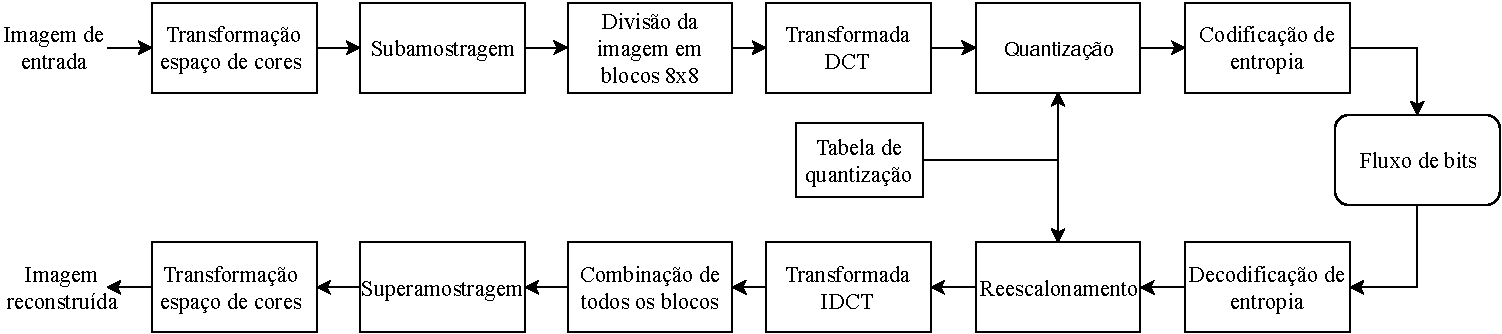
\includegraphics[width=0.9\textwidth]{figuras/jpeg.pdf}
	\caption[Padrão \acrshort{jpeg}]{Etapas da codificação e decodificação de uma imagem através do \acrshort{jpeg}.}
	\label{fig:jpeg}
\end{figure}


\subsection{Métricas de Qualidade} 

As métricas de qualidade são utilizadas para avaliar a fidelidade entre a informação que passou por um processo de compressão com perdas com a informação original.  A qualidade visual é inerentemente subjetiva e, portanto, é influenciada por muitos fatores subjetivos que dificultam a obtenção de uma medida de qualidade completamente precisa \cite{richardson2010h}.  Em imagens, as principais métricas objetivas (calculadas automaticamente) são a \gls{psnr}, \gls{ssim} e \gls{msssim} \cite{richardson2010h}. As duas últimas são métricas que levam em consideração a percepção humana.  


\subsubsection{PSNR}

A \acrshort{psnr} depende do valor máximo teórico de um pixel (255 para imagens de 8 bits) e do \gls{mse} entre a imagem original e a sua versão reconstruída. Para uma imagem monocromática $x$ de dimensões $n \times m$ representada por $P$ bits e sendo $x'$ a sua reconstrução, teremos:

\begin{equation}
\begin{aligned}
\centering    
MSE(x,x') = \displaystyle\frac{1}{nm}\sum_{i=0}^{n-1} \sum_{j=0}^{m-1} (x(i,j) - x'(i,j))^2
\end{aligned}
\end{equation} 

\begin{equation}
\begin{aligned}
PSNR_{dB}(x,x') = 10 \log\frac{(2^{P} - 1)^{2}}{MSE(x,x')} 
\end{aligned}
\end{equation}

%Um valor alto de \acrshort{psnr} indica, geralmente, uma alta semelhança perceptual entre as imagens.

\subsubsection{SSIM}
O \acrshort{ssim} foi projetado para modelar qualquer distorção da imagem como uma combinação da perda de correlação, distorção da luminância e do contraste \cite{hore2010image}. Ele é definido por:

\begin{equation}
\begin{aligned}
SSIM(x,x') = l(x,x') \times c(x,x') \times s(x,x') 
\end{aligned}
\end{equation}
Onde

\begin{equation}
\label{eq:ssim2}
\begin{aligned}
l(x,x') &= \frac{2\mu_x\mu_{x'} + C_1}{\mu_{x}^2+\mu_{x'}^2 + C_1} \\
c(x,x') &= \frac{2\sigma_x\sigma_{x'} + C_2}{\sigma_{x}^2+\sigma_{x'}^2 + C_2} \\
s(x,x') &= \frac{\sigma_{xx'}+ C_3}{\sigma_{x}\sigma_{x'} + C_3}	
\end{aligned} 
\end{equation}


O primeiro termo em \ref{eq:ssim2} é a função que mede a proximidade da luminância média de duas imagens \cite{hore2010image}. Os valores de $\mu_x$ e $\mu_{x'}$ são as médias das imagens $x$ e $x'$ que podem ser vistas como estimativas das luminâncias \cite{wang2003multiscale}. 

O segundo é a função de comparação de contraste entre duas imagens \cite{hore2010image}. Aqui, o contraste é aproximado pelo desvio padrão $\sigma_x$ e $\sigma_{x'}$.
O terceiro termo é a função de comparação de estrutura que mede o coeficiente de correlação entre as duas imagens $x$ e $x'$ \cite{hore2010image}. O termo $\sigma_{xx'}$ é a covariância entre as imagens.  As constantes positivas $C_1$, $C_2$ e $C_3$ são usadas para evitar um denominador nulo.
O \acrshort{ssim} varia de 0 a 1, onde 0 significa que não existe similaridade estrutural, e 1 significa que a similaridade estrutural é máxima, isto é, $x = x'$.


\subsubsection{MS-SSIM}
O \acrshort{msssim} \cite{wang2003multiscale} é uma variação do \acrshort{ssim} para várias escalas de imagem e conveniente para incorporar detalhes das imagens em diferentes resoluções. A imagem original e a reconstruída estão na escala 1. As imagens na escala 2 são obtidas após aplicar um filtro passa-baixas nas imagens da escala 1 (escala anterior). Esse filtro realiza subamostragem nas imagens por um fator de 2 \cite{wang2003multiscale}. Esse processo se repete até obtermos as imagens de escala $M$. 
Essas imagens são usadas para compor o cálculo do \acrshort{msssim}. Essa métrica retorna valores entre 0 (ausência de similaridade) e 1 (reconstrução sem perdas). 